\section{Wave Functions, Energies, and Observables}

\noindent For the rest of the tutorial, we will try to visualize wave functions and their associated energies in the case of the infinite well, recalling and developing points that have been addressed in class. \\ \\
Go to: \url{http://prd-mecaqu.centralesupelec.fr/FR/ex1.html}.\\ \\
\underline{Instruction}: Uncheck the "Afficher la probabilité" box. \\ \\
We provide again the wave functions and energies of a particle in an infinite potential well, as you established in Tutorial 2 of Physics:

\begin{equation}
    \phi_n(x) = \sqrt{\frac{2}{a}}\sin(\sqrt{\frac{2mE_n}{\hbar^2}}x)~~ \text{and} ~~ E_n = \frac{\hbar^2n^2\pi^2}{2ma^2}.
\end{equation}

\subsection{Wave Function and Probability Density}

\noindent \textbf{1.a)} Express, in terms of $\phi_n$, the probability of finding the particle on the interval $[x, x + dx]$.\\

\begin{breakbox}
    \noindent By definition of the probability density:
    $$\boxed{\text{d}P = \vert \phi_n(x) \vert^2 \text{d}x.}$$
\end{breakbox}

\medskip

\noindent \textbf{1.b)} Give the probability of finding the particle outside the infinite well $P_1$, and the probability of finding it within the well $P_2$, i.e., between $[0, a]$. We recall that $\displaystyle \int_{0}^{b} \sin^{2}(x) \mathrm{d}x = \frac{b}{2} - \frac{\sin(2b)}{4}.\\

\begin{breakbox}
    \noindent We have, outside of $[0, a]$:
    $$
    \boxed{P_1 = \int_{\mathbb{R} \setminus [0,a]} |\phi_n(x)|^2 \, \mathrm{d}x = 0}
    $$
    because $\vert \phi_n(x) \vert^2 = 0.$\\ \\
    Then,
    \begin{align*}
    P_2 &= \int_{0}^{a} |\phi_n(x)|^2 \, \mathrm{d}x \\
    &= \int_{0}^{a} \frac{2}{a}\sin^2\left(\sqrt{\frac{2mE_n}{\hbar^2}}x\right) \mathrm{d}x \\
    &= \int_{0}^{a} \frac{2}{a}\sin^2\left(\frac{n\pi}{a}x\right) \mathrm{d}x \\
    &= \frac{2}{n\pi} \int_{0}^{n\pi} \sin^2(y) \mathrm{d}y \\
    &= \frac{2}{n\pi}\left(\frac{n\pi}{2} - \frac{\sin(2n\pi)}{4}\right).
\end{align*}
\noindent So
    \[
        \boxed{P_2 = 1.}
    \]
\noindent This is a result that we could have expected since the particle remains confined in the well; we cannot find it outside. Thus, it only exists within $[0, a]$, and therefore $P_2 = 1$.
\end{breakbox}

\subsection{Boundary Conditions}

\noindent \textbf{2.a)} Given the probability density conditions found above, give the boundary conditions of the well for the wave function $\phi_n$. \\

\begin{breakbox}
    \noindent As seen in class, we have:
    \[
    \boxed{\phi_n(0) = 0 \text{ and } \phi_n(a) = 0.}
    \]
\end{breakbox}

\medskip

\noindent \textbf{2.b)} On the website, go to the "Wave function" section. What do you notice about the derivative of $\phi_n$ at the boundaries of the well? \\

\begin{figure}[H]
    \centering
    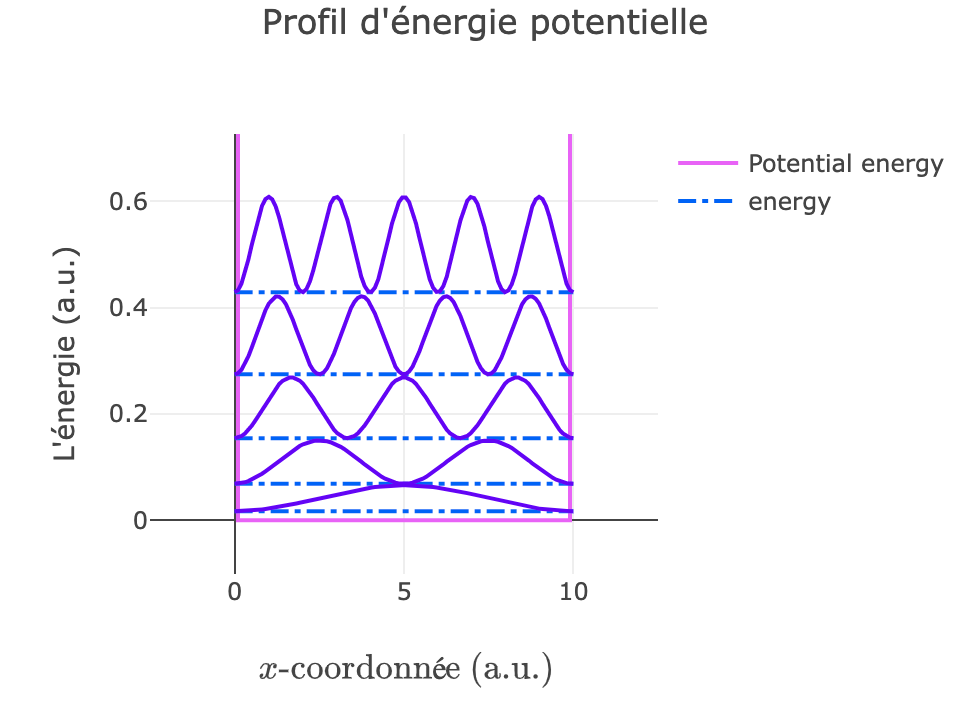
\includegraphics[width=10cm]{PI.png}
    \label{fig:enter-label}
\end{figure}

\begin{breakbox}
\noindent We notice that $\phi_n'$ seems to be discontinuous at the potential discontinuities, i.e., at $x=0$ and $x=a$. It is important to emphasize the boundary conditions and to play with the width and height of the well. For example, increasing the width decreases the energy for a given mode.\\ \\
\textit{General rule: $\phi'$ is continuous at finite potential discontinuities, is often not continuous at infinite discontinuities.}
\end{breakbox}

\medskip

\noindent \textbf{2.c)} Mathematically find the discontinuity of the derivative of $\phi_n$ (compute $\phi_n'(0+)$ and conclude).\\

\begin{breakbox}
    \noindent We have $$\phi_n'(x) = \sqrt{\frac{4mE_n}{a\hbar^2}}\cos\left(\sqrt{\frac{2mE_n}{\hbar^2}}x\right).$$ 
    \noindent Thus,
    $$\boxed{\phi_n'(0^+) = \sqrt{\frac{4mE_n}{a\hbar^2}} \neq \phi_n'(0^-) = 0.}$$    
\end{breakbox}

\medskip

\noindent \textbf{2.d)} Change and switch to "square potential" mode and see what has changed.\\

\begin{figure}[H]
    \centering
    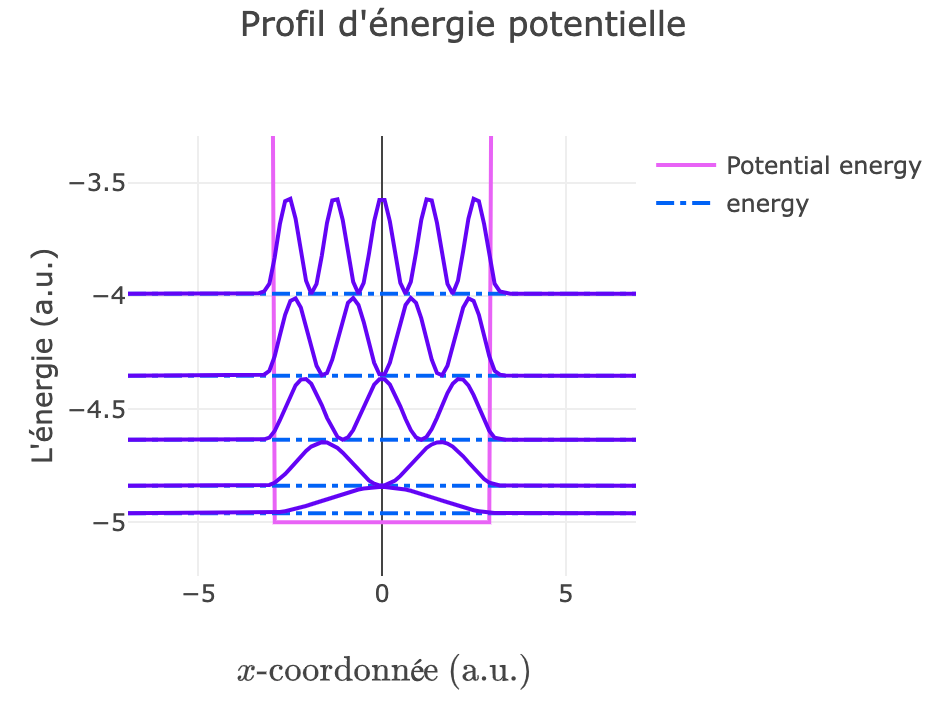
\includegraphics[width=11cm]{PF.png}
    \label{fig:enter-label}
\end{figure}

\begin{figure}[H]
    \centering
    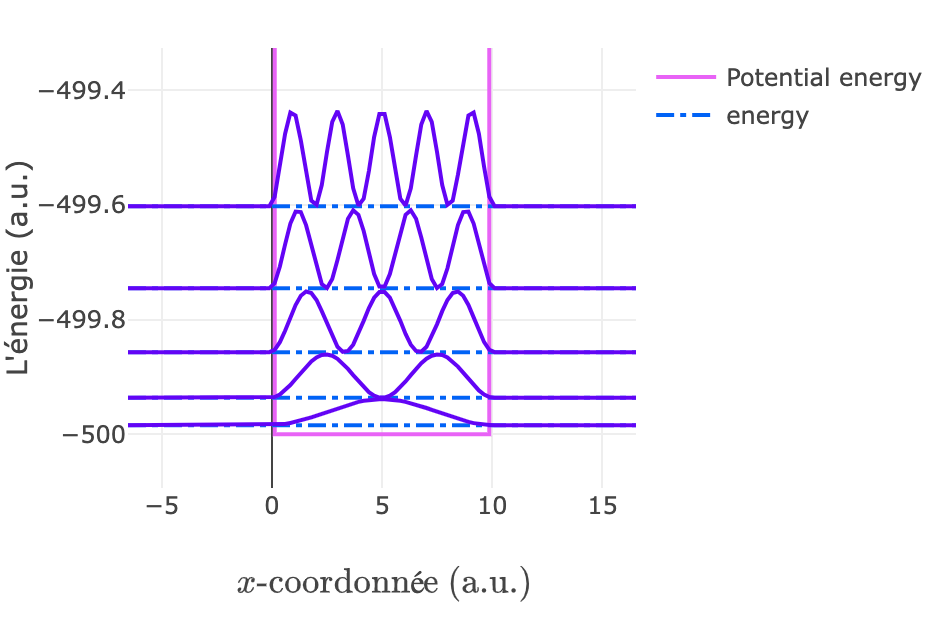
\includegraphics[width=11cm]{PF2.png}
    \label{fig:enter-label}
\end{figure}

\begin{breakbox}
    \noindent We notice that the condition of nullity at the boundaries is no longer respected. To understand concretely the transition, we can start with $V_0 = 500$: then we see that the wave functions are almost the same as in the case of the infinite well. In particular, the wave functions are zero at the boundaries and their derivatives seem to be discontinuous there. \\ \\
    If we now switch to $V_0 = 5$, we notice that the condition of nullity at the boundaries is no longer respected. In fact, inside the well, we still have sinusoidal solutions, but outside the well, we have real decreasing exponentials (make the link with the two types of solutions found in exercise 1 of this tutorial). In this situation, we also see that the derivative at the boundaries of the wave functions is now continuous.    
\end{breakbox}

\medskip

\medskip

\noindent To understand what happens when the well is finite, we consider the part $x>0$. We then consider a particle with energy $E$ coming from $x<a$. It encounters a potential barrier $U_0>E$ at $x=a$.\\

\noindent \textbf{2.e)} Determine the form of the wave functions $\psi(x,t)= \phi(x) e^{-i \frac{Et}{\hbar}}$ for $x>a$.\\

\begin{breakbox}
    \noindent We apply the Schrödinger equation to $\psi(x,t)= \phi(x) e^{-i \frac{Et}{\hbar}}$. For $x>a$, we must take into account the potential $U_0$, so the Schrödinger equation is:
    \begin{equation*}
        i\hbar\frac{\partial\psi(x,t)}{\partial t}= -\frac{\hbar ^2}{2m}\frac{\partial^2\psi(x,t)}{\partial x^2}+U_0\psi(x,t)  
    \end{equation*}

    \noindent By applying the result obtained in the first exercise, we obtain the differential equation for $\phi$:

    \begin{equation*}
        \phi^{''}(x)+\frac{2m(E-U_0)}{\hbar^2}\phi(x)=0.
    \end{equation*}

    \noindent $\displaystyle E-U_0<0$; so, by setting $\displaystyle k_{2}=\frac{2m(U_0-E)}{\hbar^2}$, we obtain a solution of the form :
    $$\phi(x) = Ce^{-k_{2}x} + De^{k_{2}x}.$$

    \noindent Since the solution cannot diverge at +$\infty$, we must have $D=0$, so we obtain the following solution:
    $$\boxed{\phi(x) = Ce^{-k_{2}x} \text{ then } \psi(x,t) = Ce^{k_{2}x}e^{\frac{-iEt}{\hbar}}.}$$

    \noindent The solution is an evanescent wave: it is a wave that does not propagate and decreases.

    \begin{figure}[H]
        \centering
        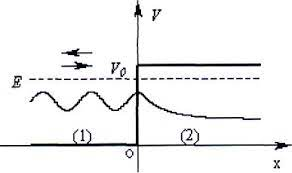
\includegraphics[width = 7cm]{Ondes_evanescentes.jpeg}
        \caption{Evanescent wave}
        \label{fig:enter-label}
    \end{figure}

    \noindent \textit{Remark: In the well for $0<x<a$, the wave function is of the form:}
    
    $$\phi(x) = A \sin(\sqrt{\frac{2mE}{\hbar^2}}x)+B \cos(\sqrt{\frac{2mE}{\hbar^2}}x).$$
    
    \noindent \textit{For $x<0$, by applying the same method as before,}
    
    $$\phi(x) = Fe^{k_{2}x}.$$
    
    \noindent \textit{To determine A, B, C, and F, we use the continuity of $\phi(x)$ and its derivative at $x=0$ and $x=a$ (see Tutorial 2 on tunneling microscope).}
\end{breakbox}

\subsection{Heisenberg's Uncertainty Principle (Bonus)}

\noindent \textbf{3.a)} Recall Heisenberg's uncertainty principle by redefining the two terms involved.\\

\begin{breakbox}
    \noindent Heisenberg's uncertainty principle, or the uncertainty principle, is written as follows:
    \[
        \boxed{\sigma_x\sigma_p \ge \frac{\hbar}{2}.}
    \]
    \noindent We recall that  
    $$\sigma_x^2 = \langle X^2 \rangle_{\psi} - \langle X \rangle_{\psi}^2 \text{ and } \sigma_p^2 = \langle p^2 \rangle_{\psi} - \langle p \rangle_{\psi}^2.$$
    \noindent And in general, for any operator A: 
    $$\boxed{\langle A \rangle_{\psi} = \int \psi^* A \psi \operatorname{dP}.}$$
\end{breakbox}

\medskip

\noindent \textbf{3.b)} Calculate $\langle X \rangle_{\phi_n}$ using the wave functions of the infinite quantum well. \\

\begin{breakbox}
    \noindent We have
    \begin{align*}
        \langle X \rangle_{\phi_n} &= \int_{0}^{a} \phi_n^{*} x \phi_n \mathrm{d}x \\
        &= \int_{0}^{a} \frac{2}{a}x\sin^{2}\left(\sqrt{\frac{2mE_n}{\hbar^2}}x\right) \mathrm{d}x \\
        &= \int_{0}^{a} \frac{2}{a}x\sin^{2}\left(\sqrt{\frac{n\pi}{a}}x\right) \mathrm{d}x \\
        &= \frac{2a}{n^2\pi^2} \int_{0}^{n\pi} X \sin^{2}(X) \mathrm{d}X.
    \end{align*}
    \noindent By making the change of variable $\displaystyle \frac{n\pi}{a}x = X$.\\ \\
    \noindent We calculate separately, using integration by parts (the result can be given to the students):
    \begin{align*}
        \int_{0}^{b} x\sin^{2}(x) \, \mathrm{d}x &= \int_{0}^{b} x\left(\frac{1-\cos(2x)}{2}\right) \, \mathrm{d}x \\
        &= \left[x \frac{x - \frac{\sin(2x)}{2}}{2}\right] - \int_{0}^{b} x - \frac{1}{2}\sin(2x) \, \mathrm{d}x \\
        &= \frac{b^2}{2} -\frac{b}{4}\sin(2b) - \frac{b^2}{4} +\frac{1}{4}\left[-\frac{\cos(2x)}{2}\right

] \\
        &= \frac{b^2 - b\sin(2b) + \frac{1-\cos(2b)}{2}}{4}.
    \end{align*}

    \noindent Finally:
    $$\boxed{\langle X \rangle_{\phi_n} = \frac{2a}{n^2\pi^2}\frac{n^2\pi^2}{4} = \frac{a}{2}.}$$
\end{breakbox}

\medskip

\noindent \textbf{3.c)} Verify on the website that the inequality is satisfied.\\

\begin{breakbox}
    \noindent On the website, go to the "Observables" tab at the bottom of the page, then choose "Heisenberg Uncertainty Principle" from the dropdown menu. We can see that the curve remains above $\displaystyle \frac{\hbar}{2}$.
\end{breakbox}

\medskip

\noindent \textbf{3.d)} Discuss the physical interpretation of this inequality by relating it to its name of uncertainty principle.\\

\begin{breakbox}
    \noindent This inequality shows that there is a theoretical limit to the precision with which two physical properties of the same particle can be simultaneously known. For example, the better the measurement of position, the less precise the measurement of momentum will be, and vice versa.    
\end{breakbox}